\documentclass[11pt]{article}
\usepackage{hyperref}
\usepackage{amsmath, amsfonts, amssymb, mathrsfs, dsfont}
\usepackage{dcolumn}
\usepackage{caption}
\usepackage{subcaption}
\usepackage{filemod}
\usepackage{natbib}
\usepackage[ruled, vlined]{algorithm2e}
\usepackage{floatrow}
\usepackage{setspace}
\usepackage{verbatim}
\usepackage{graphicx}
\usepackage{bbm} % for indicator function
\usepackage{xcolor} % only for coloring text while revising

\usepackage{tikz} % for pretty diagonal matrix
\usetikzlibrary{matrix,decorations.pathreplacing,calc}

\hypersetup{
    colorlinks=true,
    linkcolor=blue, 
    urlcolor=black,
    citecolor=blue, 
    }

\oddsidemargin=0.25in
\evensidemargin=0.25in
\textwidth=7in
\textheight=8.75in
\topmargin=-.5in
\addtolength{\oddsidemargin}{-.5in}
\addtolength{\evensidemargin}{-.5in}
\footskip=0.5in
%\doublespacing

\title{Bayesian Deep Gaussian Processes for Correlated Functional Data: \\
        A Case Study in Cosmological Power Spectra}
\author{Stephen A. Walsh\thanks{Corresponding author: Division of Natural Sciences, 
        Math and Technology, Elms College, {\tt walshst@elms.edu}} \and 
        Annie S. Booth\thanks{Department of Statistics, Virginia Tech} \and
        David Higdon\footnotemark[2] \and
        Marco A.R. Ferreira\footnotemark[2] \and
        Jared Clark\footnotemark[2] \and
        Kelly Moran\thanks{Los Alamos National Laboratory} \and
        Katrin Heitmann\thanks{Argonne National Laboratory}}
\date{\today}


\begin{document}

\maketitle
\bigskip

\begin{abstract} 
Understanding the structure of our universe and the distribution of matter is an 
area of active research.  As cosmological surveys grow in complexity, the development 
of emulators to efficiently and effectively predict matter power spectra is essential.  
We are particularly motivated by the Mira-Titan Universe simulation
suite which, for a specified cosmological parameterization (termed a ``cosmology''), 
provides multiple response curves of various fidelities, including correlated 
functional realizations.  Our objective is two-fold.  First, we estimate 
the underlying true matter power spectra, with appropriate uncertainty 
quantification (UQ), from all of the provided curves.  To this end, we propose a 
novel Bayesian deep Gaussian process (DGP) hierarchical model which synthesizes 
all the simulation information to estimate the underlying matter power spectra
while providing effective UQ.  Our model extends previous work on Bayesian DGPs 
from scalar responses to functional ones.  Second, we leverage our predicted 
power spectra from various cosmologies in order to accurately predict the entire 
matter power spectra for an 
unobserved cosmology.  For this task, we use basis function representations 
of the functional spectra to train a separate Gaussian process emulator.  
Our method performs well in synthetic exercises and against the benchmark cosmological 
emulator (Cosmic Emu).
\end{abstract}

\noindent \textbf{Keywords:} computer experiment, Cosmic Emu, 
principal components analysis, Mira-Titan, surrogate, uncertainty quantification

%\vfill

\section{Introduction}
%%%%%%%%%%%%%%%%%%%%%%%%%%%%%%%%%%%%%%%%%%%%%%%%%%%%%%%%%%%%%%%%%%%%%%%%%%%%%%%

%To further our understanding of the structure and movement of the universe, 
%researchers utilize numerous cosmological surveys such as the Sloan Digital Sky 
%Survey \citep{york2000sloan} and the upcoming Nancy Grace Roman Space Telescope 
%\citep{Dore2019WFIRST} which are continuously growing in complexity. With these 
%tools, cosmologists aim to continue learning more about cosmic acceleration 
%\citep{caldwell2009physics}. To this end, one important ingredient to aid in this 
%understanding of our universe is the matter power spectrum. 

Computer simulation experiments are invaluable tools in the study of cosmology.
Experiments which simulate the expansion of the universe are growing
in prevalance and complexity \citep[e.g.,][]{lawrence2010coyote,derose2019aemulus,
nishimichi2019dark,angulo2021bacco,euclid2021euclid,moran2023mira}.  
We are particularly motivated by a simulation
of the matter power spectrum, which describes the distribution of matter as a 
function of spatial scale. 
%It is often represented as a function of wavenumber $k$ (units Mpc$^{-1}$), which is 
%inversely related to spatial scale. 
On large scales, power spectrum behave according to linear perturbation 
theory \citep{pietroni2008flowing, lesgourgues2009non}.  On smaller scales, nonlinear 
dynamics require the use of computationally intensive simulations, yielding
correlated functional data.
%the Coyote Universe \citep{lawrence2010coyote} and the Mira-Titan Universe \citep{moran2023mira} 
%are two simulation suites dedicated to this effort.  
Our overarching goal is to leverage such simulation data to 
first estimate and then predict underlying power matter spectra for various 
cosmological parameterizations.

The Mira-Titan simulation suite \citep{moran2023mira}
defines ``cosmologies'' according to eight cosmological parameters (more on this
in Section \ref{sec:data}).  For a particular cosmology, the simulation of the power matter spectra 
is rather complex.  Although we presume there exists some true matter spectra as a function
of wavenumber, we are not able to directly observe it.  Rather, the simulation returns
a convoluted patchwork of potential spectra, which vary in fidelity and are only trusted
over particular wavenumber ranges.  Our first objective is to synthesize expert knowledge
and all available simulation information into an effective estimate of the true underlying
matter spectrum.  

There are several challenges to estimating the underlying spectra.  Our model
must: handle multiple correlated functional observations, offer enough 
flexibility to accommodate the nonstationarity present in power matter spectra 
(which vary in smoothenss across wavenumbers), provide effective uncertainty
quantification (UQ), and allow for the incorporation of expert knowledge 
regarding the wavenumbers over which various outputs are trusted.  To this end, 
we propose a Bayesian hierarchical model which treats functional simulation 
outputs as realizations of a deep Gaussian process \citep[DGP;][]{damianou2013deep} 
centered on the true underlying spectra.  The hierarchical structure naturally
accommodates the correlated observations.  The depth of the DGP offers nonstationary
flexibility.  The Bayesian framework facilitates UQ and the incorporation of prior
knowledge.  While Bayesian DGPs have been previously deployed for computer experiments 
with scalar responses \citep[e.g.,][]{sauer2023active,sauer2023vecchia,ming2023deep}, 
they have yet to be extended to correlated functional outputs. 
To demonstrate the profiency of our Bayesian hierarchical DGP, 
we benchmark its performance in two unique settings: with synthetic data 
mimicing the Mira-Titan data and with real-world data from 
the Code for Anisotropies in the Microwave Background \citep[CAMB;][]{lewis2011CAMB}.
The CAMB model also exhibits similar behavior to Mira-Titan, but crucially
provides a ``true" power spectrum corresponding to each cosmology.

Our second objective is to leverage simulation data from a limited set of
cosmologies in order to predict power matter spectra for unobserved cosmologies.
Due to the computationally expensive nature of the Mira-Titan simulation suite
(one batch of simulations can take multiple weeks to run on a supercomputer),
it is infeasible to evaluate the simulation for every possible eight-dimensional
cosmological configuration which may be of interest.  Instead, we desire
a statistical ``emulator'' or ``surrogate model'' 
\citep{santner2003design,gramacy2020surrogates} which will provide quick and effective
predictions of power matter spectra for any cosmological parameterization.
\citet{moran2023mira} provide a state-of-the-art emulator for the Mira-Titan
simulation suite, which was trained on 117 simulations, and is termed 
the ``Cosmic Emu.''\footnote{\url{https://github.com/lanl/CosmicEmu}}
We leverage the same training data, in conjunction with our Bayesian hierarchical
DGP model and basis function representations, to train a Gaussian process surrogate 
on principal component weights in order to predict spectra for unobserved
cosmologies \citep{higdon2008computer, higdon2010estcosmo}. 
Our method compares favorably to Cosmic Emu on held-out cosmologies.

The remainder of the paper is organized as follows.  Section \ref{sec:data} 
introduces our motivating application, the Mira-Titan simulation suite.  
Section \ref{sec:hm_fit} describes our hierarchical Bayesian DGP and 
validates its performance on synthetic exercises and the CAMB simulations.  
Leveraging this trained model, Section \ref{sec:pred} details 
our procedure for predicting at unobserved cosmologies, benchmarking against
state-of-the-art competitors on the CAMB and Mira-Titan simulations. 
Section \ref{sec:disc} concludes with a discussion of our contributions and avenues for 
future research.  We provide reproducible code and an {\sf R} package for our 
Bayesian DGP model in a public git repository.\footnote{\url{https://github.com/stevewalsh124/dgp.hm}}
\textcolor{cyan}{Please note: this repository is currently private until we 
hear back regarding permissions for sharing the Mira-Titan data alongside our code.}

%Leveraging these simulations allows for emulation and prediction of the matter power 
%spectrum under varying specifications for eight different cosmological parameters 
%(i.e., different cosmologies). Estimating and understanding the influence of these 
%parameters on cosmic expansion are areas of active research. In addition to 
%presenting the Mira-Titan simulation suite, \cite{moran2023mira} builds off 
%of previous spectrum emulation \citep{lawrence2017mira} to provide the final 
%emulator (Cosmic Emu) based on the full suite of 117 batches of simulations. 

%In this work, we expand on the previous emulation approaches and propose a 
%novel synthesis of methods to quantify uncertainty and predict matter power 
%spectra for different cosmologies using deep Gaussian processes (DGPs). In order 
%to handle multiple realizations of functional output (from the Mira-Titan 
%simulation suite), we use hierarchical modeling and basis functions within our 
%DGP framework to accurately estimate and predict power spectra for different 
%cosmologies. 

\section{Mira-Titan}
\label{sec:data}

The Mira-Titan simulation suite is a dataset consisting of simulated power spectra for 
117 different cosmologies. Each of these cosmologies is specified by eight cosmological 
parameters: matter density, baryon density, amplitude of density fluctuations, 
dimensionless Hubble parameter, spectral index of scalar perturbations,
dark energy equation of state parameters, and neutrino density. For more details 
on these parameters and their effects, see \cite{dodelson2020modern, aghanim2020planck, heitmann2016mira}. 
Parameter ranges are specified in Table 2.1 of \cite{moran2023mira}.
There is an optional ninth parameter, the redshift, which we fix at 0.
%Different simulation output exists for different values of a ninth value, 
%the redshift; in this work, we fix 
%this value at 0. 

% after \linewidth:, trim=0 13 0 45, clip=TRUE
\begin{figure}[ht]
    \centering 
    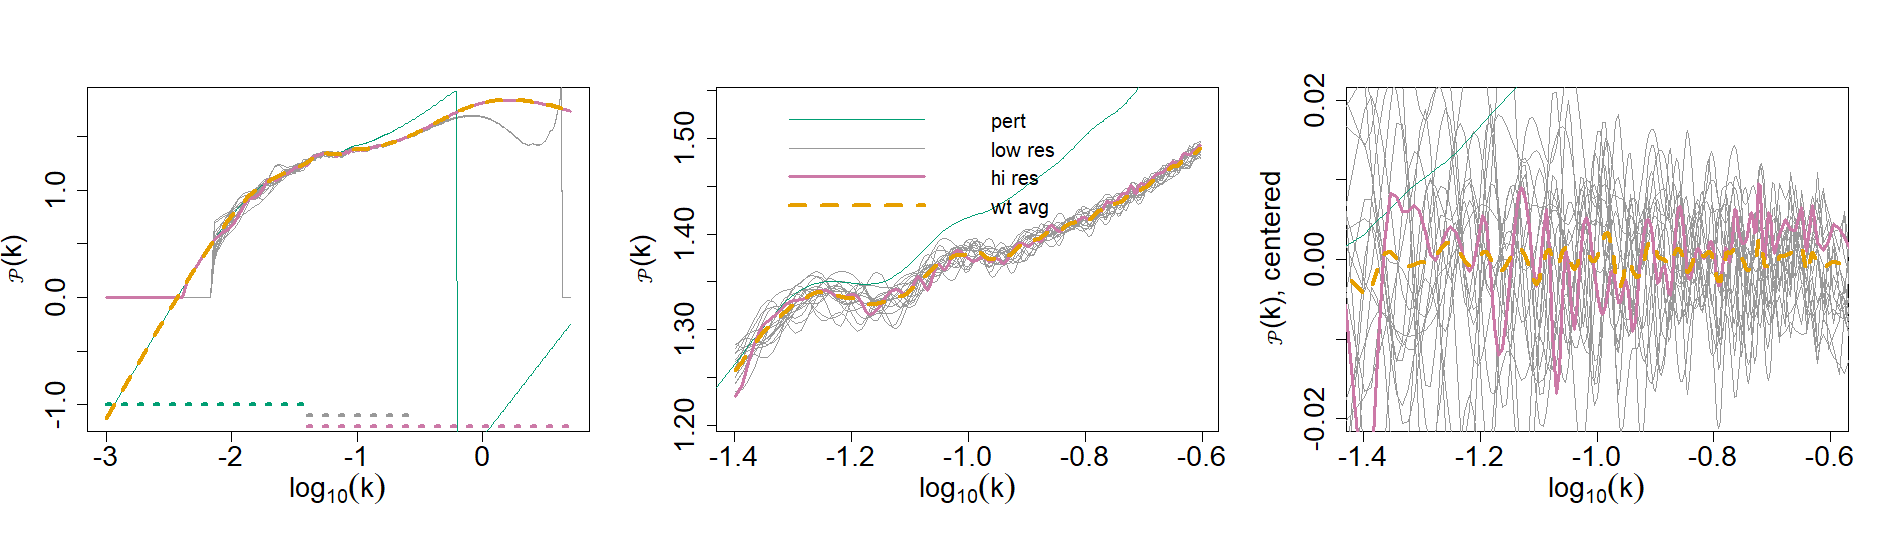
\includegraphics[width=\linewidth]{plot_data.png}
    \caption{{\it Left:} The perturbation theory (solid green), low resolution runs (solid grey), 
    and high resolution run  (solid pink) for a particular cosmology. 
    The weighted average of these is shown in dashed orange. Dotted lines at the bottom 
    indicate where each data type is deemed approximately unbiased. 
    {\it Middle:} Same as left, but restricted to wavenumber ($k$) values where the low resolution 
    runs are approximately unbiased.
    {\it Right:} Same as middle, but with estimated posterior mean subtracted.}
    \label{fig:plot_data}
\end{figure}

For each cosmology, Mira-Titan contains a batch of 18 simulated spectra: an inexpensive 
spectrum estimated from linear perturbation theory ($y_p$), 16 spectra estimated from 
lower resolutions simulations ($y_{\ell_r}, r \in \{1,\dots,16\}$), and one spectrum from 
a high resolution simulation ($y_h$). 
These spectra are represented as a function of wavenumber $k$.  Following 
\cite{moran2023mira}, we model on the emulation space 
$\mathcal{P}(k)=\log_{10}\left(\frac{k^{1.5}P(k)}{2\pi^2}\right)$, where $P(k)$ represents the
original spectra. Output is available for $n=351$ values of $k$, spanning
$0.001 \leq k \leq 5$, but each data type has unique wavenumber ranges
where it is deemed approximately unbiased. For $k<0.04$, only $y_p$ provides a reliable 
estimate of the true spectra. $y_{\ell_r}$ are valid for $0.04 \leq k \leq 0.25$, and 
$y_h$ is valid for $0.04 \leq k \leq 5$.  Figure \ref{fig:plot_data} shows an example 
of the output for a particular cosmology. When we focus on $k$ values where $y_{\ell_r}$ 
is valid (center panel), we see each low-resolution and the high-resolution run oscillate around 
a mean term, which is relatively smooth, compared to these realizations. When this
mean term is subtracted, we will obtain a plot like the right panel in 
Figure \ref{fig:plot_data}.

Notice, in the center/right panels of Figure \ref{fig:plot_data}, the precision of each
low/high resolution spectra increases as $k$ increases.  The curves get progressively 
tighter from left to right.  We would like to conveniently wrap this domain-specific 
knowledge inside our Bayesian framework later.  To this end, \cite{moran2023mira} 
used the multiple low- and high-resolution spectra across all cosmologies to
obtain precision estimates, $p_1,\dots, p_n$, across the $n$ 
wavenumber values using a log-log regression model. A multiplier $c$ for 
the increase in precision from the low- to high- resolution output is also 
estimated with this regression model. We use these estimates to define three 
diagonal precision matrices, one for each data type (perturbation theory, 
low resolution average, and high resolution). Specifically, denote $\Lambda_p$, 
$\Lambda_\ell$, and $\Lambda_h$ as the $n\times n$ diagonal matrices with elements
\[
\Lambda_p^{(ii)} = \begin{cases}
    10^5 &\text{for } k_i < 0.04 \\
    0  &\text{otherwise}\\
    \end{cases}
\quad
\Lambda_\ell^{(ii)} = \begin{cases}
    16p_i &\text{for } 0.04 \leq k_i < 0.25 \\
    0  &\text{otherwise}\\
    \end{cases}
\quad
\Lambda_h^{(ii)} = \begin{cases}
    cp_i &\text{for } 0.04 \leq k_i < 5 \\
    0  &\text{otherwise}\\
    \end{cases}
\]
for $i=1,\dots, n$.  In $\Lambda_p$, we use the sufficiently high precision 
of $10^5$ to impose the deterministic nature of the perturbation theory output.
In $\Lambda_\ell$, the multiplication by 16 accounts for the sample size of the
low resolution runs.
We then calculate a weighted average for each cosmology: 
$\bar y = \Lambda^{-1}(\Lambda_p y_p + \Lambda_{\ell} \bar{y}_\ell + \Lambda_h y_h)$, 
where $\Lambda = \Lambda_p + \Lambda_\ell + \Lambda_h$ and 
$\bar{y}_\ell = \frac{1}{16}\sum_{r=1}^{16} y_{\ell_r}$. In Figure \ref{fig:plot_data},
the weighted average is shown in dashed orange.  As an estimate of the true
underlying spectrum, the weighted average fluctuates too drastically due 
to the limited amount of data.  It fails to account for the
spatial dependence inherent in the smooth but stochastic spectra,
which is pivotal to effectively inferring the true spectrum.

%We consider a training-testing split with 111 cosmologies used for estimation and 6 
%cosmologies held out for testing.  Our ultimate objective is to effectively predict
%the underlying power matter spectra for the held-out cosmologies based on their 
%8-dimensional input configuration (Section \ref{sec:pred}).  But first, we must 
%obtain effective estimates of the underlying spectrum for each training 
%cosmology (Section \ref{sec:hm_fit}). \textcolor{red}{(@Steve - maybe this is a
%good place to introduce the ``hold out'' and ``within sample'' terms?)}

\section{Bayesian Hierarchical Modeling for Particular Cosmologies}
\label{sec:hm_fit}

Here we describe our first contribution: the use of a Bayesian hierarchical model 
to estimate the underlying spectra and quantify uncertainty for a particular cosmology.
Let input $X$ represent the $n$-vector of $\log_{10}(k)$ values.
In the previous section, we used lowercase $\bar{y}$ to denote 
the observed weighted average; now, we use $\bar{Y}$ to indicate the corresponding 
random variable within the statistical model.  $\bar{Y}$ is typically pre-processed
in a domain-specific manner, such as that defined in Section \ref{sec:data}.
Together, $X$ and $\bar{Y}$ comprise the training data for a particular cosmology.
We will reserve specific integration 
of expert knowledge for the CAMB and Mira-Titan suites, such as this pre-processing,
for Sections \ref{subsec:camb} and \ref{subsec:mira_fit}, respectively.  

\subsection{Deep Gaussian Process Hierarchical Model}

Here, we introduce the Bayesian Gaussian Process (GP) model. We assume 
the matter power spectrum $S$ for a given cosmology follows a GP with mean $\mu$ 
and covariance matrix $\Sigma_S$. From the data, we obtain $\bar Y$, which is a 
noisy version of $S$.  Let $S$ represent the true (but unknown) underlying
power matter spectra from which $D$ was generated.

From plots of the multiple low-resolution spectra (e.g., Figure \ref{fig:plot_data}), 
we find they vary smoothly about some mean $S$, suggesting that a dense covariance 
matrix $\Sigma_\varepsilon$ (accounting for spatial dependence) may outperform a 
diagonal covariance $\Lambda_\ell^{-1}$ for $\bar Y$. In previous work, we have 
modeled multiple candidates for $\Sigma_\varepsilon$ \citep{walsh2023bayesian} and 
found that a Mat\'ern covariance $\Sigma_\ell$ trained on the low-resolution runs 
(pre-scaled by the precision values and subtracting a LOESS-smoothed average) performs 
the best. We specify this structure within $\Sigma_\varepsilon$ and refer readers 
to \cite{walsh2023bayesian} for a more detailed exposition. This yields 
$\Sigma_\varepsilon=\left(\Lambda_p^{-1} + \Sigma_\ell + \Lambda_h^{-1}\right)^{-1}$, 
where $\Lambda_p, \Sigma_\ell^{-1}, \text{ and } \Lambda_h$ are all $n\times n$ 
and are 0 wherever the corresponding data type is biased.

Therefore, we model $\bar Y|S$ as a GP with mean $S$ and block-diagonal covariance 
matrix $\Sigma_\varepsilon$:

\begin{align}
\bar Y|S &\sim GP\left(S,\Sigma_\varepsilon\right) \\
S &\sim GP\left(\mu, \Sigma_S(x,x')\right)
\end{align}

We transform $X$ values to fall within $[0,1]$ and $\bar Y$ so that the mean and variance 
are 0 and 1, respectively. This allows for a straightforward specification of priors, 
where the hyperparameters for the Mat\'ern covariance $\Sigma_S$ each take a vague prior. 
Specifically:

\begin{align}
\Sigma_\ell^{i,j} = \tau_\ell^2  \left( 1 + \frac{\sqrt{5}d}{\sqrt{\theta_\ell}} + 
  \frac{5d^2}{3\theta_\ell}\right) \exp\left(-\frac{\sqrt{5}d}{\sqrt{\theta_\ell}}\right),\\
\Sigma_S^{i,j} = \tau_S^2  \left( 1 + \frac{\sqrt{5}d}{\sqrt{\theta_S}} + 
  \frac{5d^2}{3\theta_S}\right) \exp\left(-\frac{\sqrt{5}d}{\sqrt{\theta_S}}\right),
\end{align}

where $d=||x_i-x_j||^2$. From here, we estimate $\tau_\ell, \theta_\ell$ with maximum 
likelihood, and conditional on $\Sigma_\varepsilon$, we specify priors for $\tau_S, \theta_S$ 
following \cite{sauer2023active}: \textcolor{red}{Annie, please ensure the most up-to-date 
prior specs are shown above and here. Here is what I found from fit\$settings when using 
deepgp v1.1.3: $\theta_S \sim G(\alpha=1.2, \beta=1)$ and $\tau_S \propto 1/\tau_S^2$.}

% $$
% \mathbf{\Sigma_\varepsilon} =
% \begin{bmatrix}
% \Lambda_p^{-1} & \mathbf{0} & \mathbf{0} \\
% \mathbf{0} & \mathbf{\Sigma}_{\ell} & \mathbf{0} \\
% \mathbf{0} & \mathbf{0} & \Lambda_h^{-1}
% \end{bmatrix}
% $$

A key property of GPs is that any finite set of $n$ observations from the GP is a 
multivariate normal distribution. Therefore, upon integrating out $S$, we obtain 
$\bar{Y} \sim \mathcal{N}_n(\mu, \Sigma_S+\Sigma_\varepsilon)$ for the $n$ observed X locations. 
Additionally, this model yields the posterior distribution $S|\bar Y \sim \mathcal{N}_n(m, C)$, 
where $C=\left(\Sigma_S^{-1}+\Sigma_\varepsilon^{-1}\right)^{-1}$ and 
$m=C\left(\Sigma_\varepsilon^{-1}\bar Y+\Sigma_S^{-1}\mu\right)$. 
This distribution provides the posterior mean and corresponding uncertainty for 
$S$ within a given cosmology. 
% With this hierarchical model, we improve the efficiency of estimating $S|\bar{Y}$.

Considering the Mira-Titan data, some nonstationarity is expected (e.g., due to 
baryonic acoustic oscillations when $-2 \leq \log_{10}(k) \leq -1$). To account 
for this, we incorporate a latent layer $W$ within the hierarchical model to warp 
locations of $X$ and incorporate nonstationary dynamics of the matter power spectra. 
When $W$ is a GP, this creates a deep Gaussian process (DGP) model \citep{damianou2013deep}. 
Additional latent layers could be considered, although one is sufficient for this 
dataset \citep{dunlop2018deep}.

\begin{align}
\bar Y|S,W &\sim \mathcal{N}_n(S,\Sigma_\varepsilon) \\
S|W &\sim GP\left(\mu, \Sigma_S(w,w')\right) \\
W &\sim GP\left(0, \Sigma_W(x,x')\right)
\end{align}

We have found that whether the prior mean of $W$ is set to 0 or $X$ 
\citep[which would indicate stationarity apriori,][]{schmidt2003bayesian} does not 
have a substantial impact on the model fit. We construct this model in the 
compositional form, and also use Markov Chain Monte Carlo (MCMC) to estimate and 
obtain full uncertainty for each of the model parameters \citep{sauer2023active}.

\textcolor{red}{Annie: want to add something here? For $\theta_w$, we also specify 
a Gamma prior of the form $\theta_w \sim G(\alpha=1.2, \beta=2)$. We discuss the 
elliptical slice sampling of $W$, but otherwise it is plugged in to the methods 
of the previous section with very few changes.}

Through the synthesis of the DGP model alongside the additional level of hierarchical 
modeling (HM) to incorporate multiple functional model runs, we call this method DGP.HM.

\subsection{Simulation Study}
\label{subsec:sim}

We compare DGP.HM to competing models with a simulation study where the underlying 
true curve is known. Following \cite{moran2024dpc}, we consider two functions 
($f_1$ and $f_2$) each with two variance specifications (settings ``4" and ``5", 
\textcolor{magenta}{we can consider additional homoskedastic cases in the appendix if necessary}). 

Here, $f_1$ and $f_2$ are defined as follows:
\begin{align}
  f_1(x) &= m_1 \exp(-u_1x/2) * \cos(wx) - m_1x/5, \quad w=\sqrt{25-[u_1/2]^2} \\
  f_2(x) &= \exp(-m_2[x-3]^2)+\exp(-u_2[x-1]^2)-0.05\sin(8[x-1.9]), \\ 
  \quad x &\in [0,4].
\end{align}

For additional variation, the values of $m_1, m_2, u_1,$ and $u_2$ are random where 
$m_1 \sim \text{Uniform}(0.5,1.5)$, $u_1 \sim \text{Uniform}(1.5,2.5)$, and $m_2,u_2 
\sim \text{Uniform}(0.6,1.4)$. 
      
For the two variance settings, we consider matrices $\Sigma_4$ and $\Sigma_5$ to 
have a Mat\'ern covariance function with a nugget of $10^{-8}$ and smoothness of 2.5. 
For setting ``4", we have $\tau^2=0.0225$ and $\theta=0.01$. For setting ``5", we have 
$\tau^2=0.01$ and $\theta=0.05$, and additionally scale this covariance matrix by 
a vector of values $s$ so that $\Sigma_5 = s M s^T$ is nonstationary; here $M$ is 
a Mat\'ern covariance matrix with parameters $\tau^2$ and $\theta$.

For each simulated function and variance specification, we generate 20 values of 
$m_1, m_2, f_1, f_2$, and conditional on these values, we sample either 5 or 20 
functional observations and estimate the underlying true function based on the observations.

\begin{figure}[t]
    \centering
    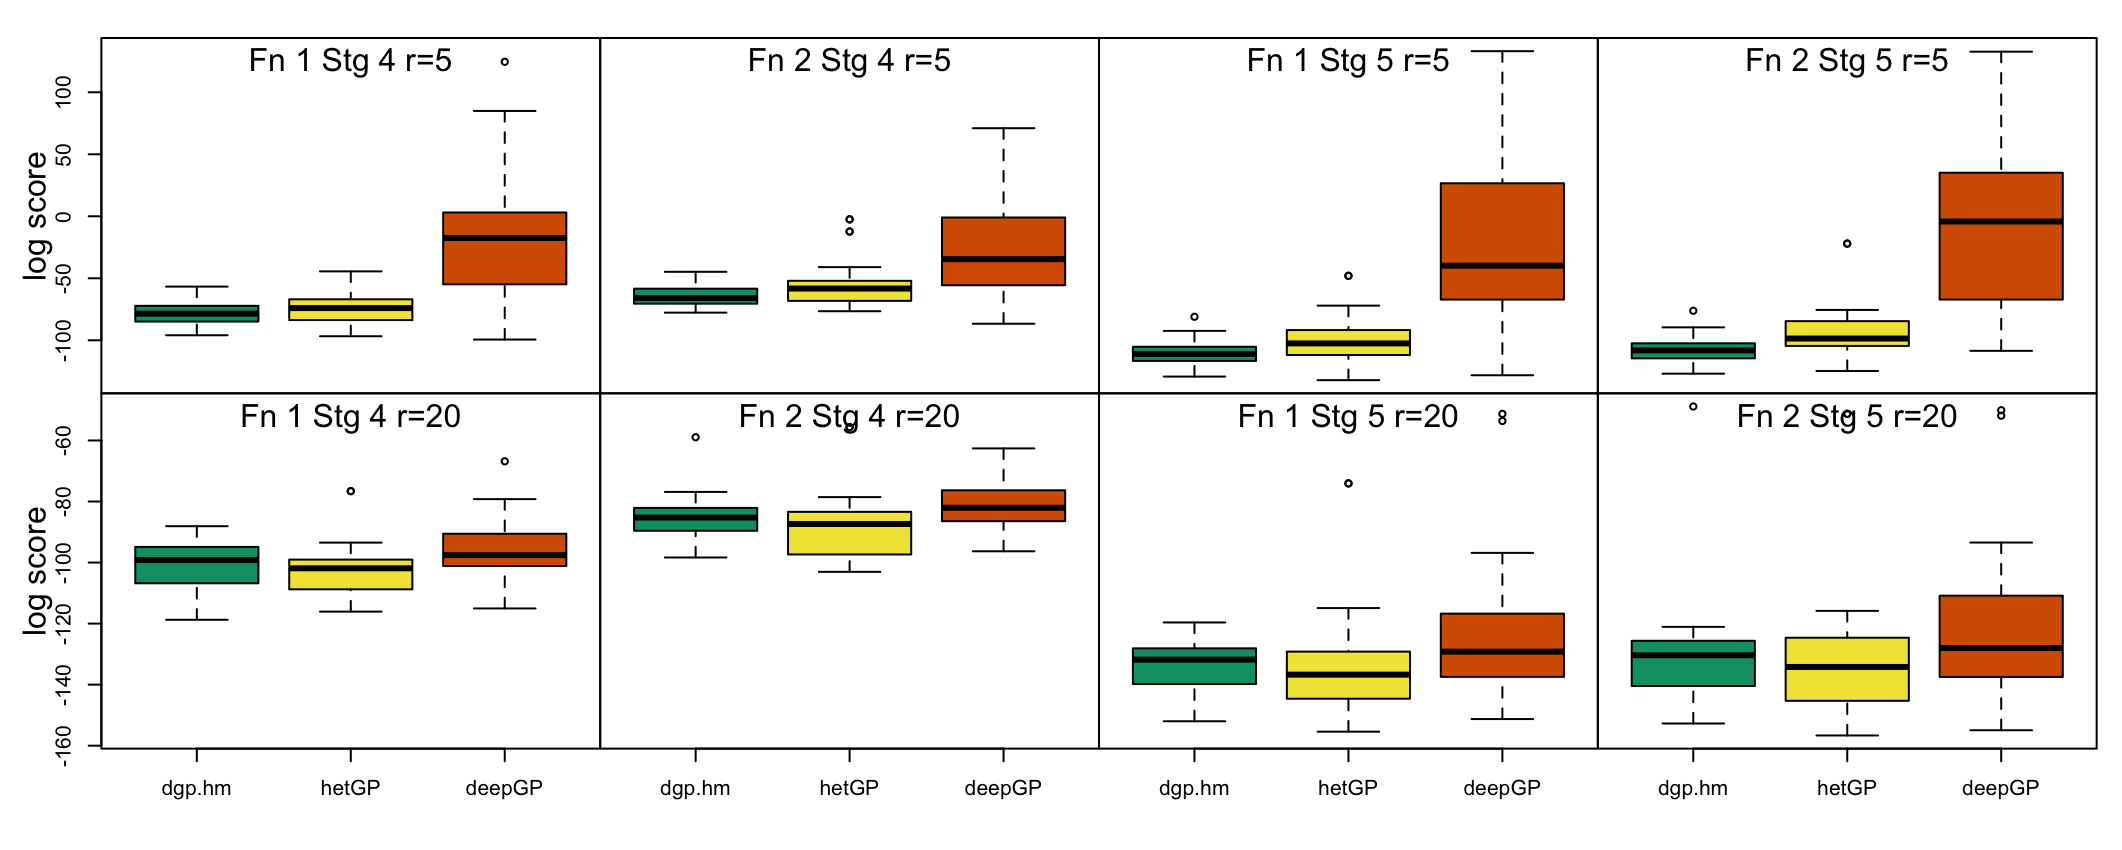
\includegraphics[width=6in]{sims_logS.png}
    \caption{Boxplot of log scores across two different functions and covariance 
             settings (lower is better). For each case, the boxplot is constructed 
             from 20 random batches were simulated. Each column represents a function/variance 
             specification pair, and each row shows results for batch sizes of either 
             5 (top) or 20 (bottom).}
    \label{fig:sims_logS}
\end{figure}

The competing methods we consider are an out-of-the-box DGP fit using the 
\texttt{deepgp} package \citep{sauer2023active}, a heteroskedastic GP fit using 
the \texttt{hetGP} package \citep{binois2018practical, binois2021hetgp}, as well 
as a deep process convolution (DPC) approach, which is utilized within Cosmic 
Emu \citep{moran2023mira}. 

The metrics we use to evaluate performance are mean squared error (MSE) and the 
log score, a proper scoring rule which takes both prediction and intervals into 
consideration \citep{gneiting2007strictly}. For both metrics, a lower value indicates 
better performance. Log score and MSE results are shown in Figures \ref{fig:sims_logS} 
and \ref{fig:sims_MSE} respectively; our DGP.HM model performs favorably against 
these current benchmark methods. \textcolor{magenta}{If we mention that DGP.HM timings 
speed up compared to \texttt{deepgp}, we would also need to mention that \texttt{hetGP} 
is much faster than both of these.}

\begin{figure}
    \centering
    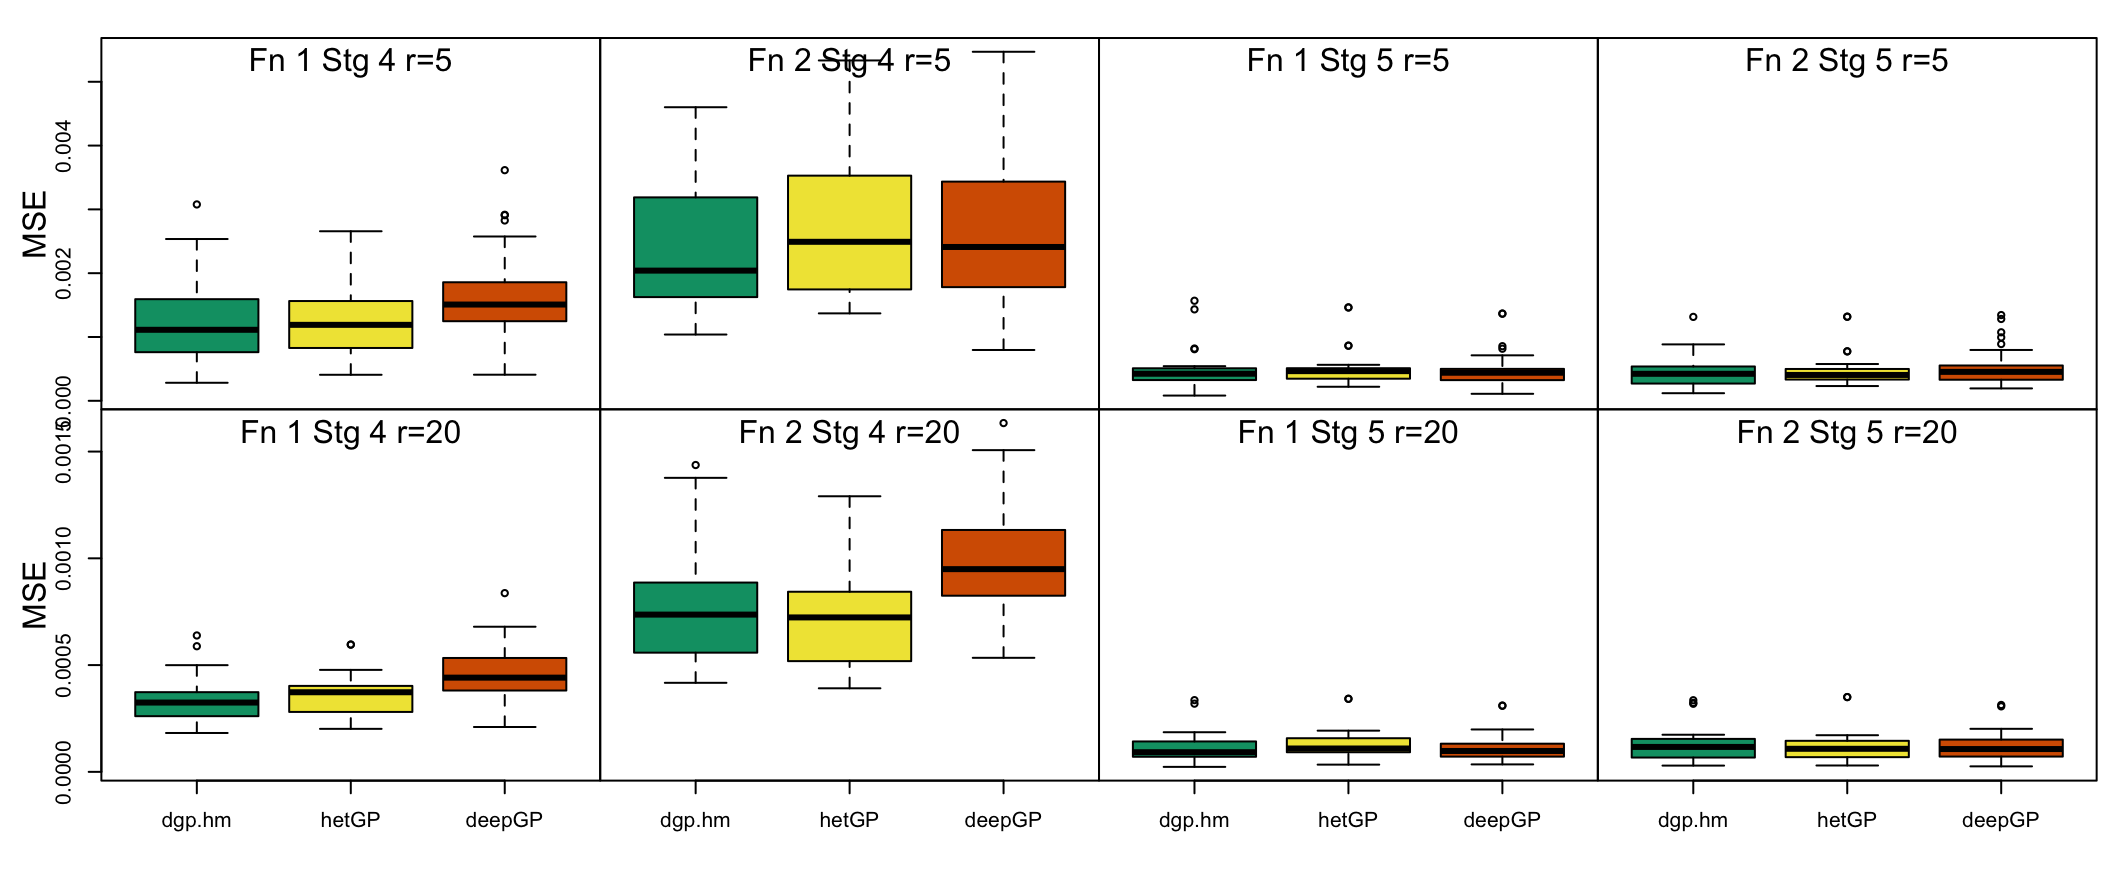
\includegraphics[width=6in]{sims_MSE.png}
    \caption{Boxplot of MSEs across two different functions and covariance settings 
             (lower is better). For each case, the boxplot is constructed from 20 
             random batches were simulated. Each column represents a function/variance 
             specification pair, and each row shows results for batch sizes of 
             either 5 (top) or 20 (bottom).}    
    \label{fig:sims_MSE}
\end{figure}

\subsection{CAMB Data}
\label{subsec:camb}

In addition to simulated data, we investigate model fits for different cosmological 
datasets from CAMB \citep{lewis2011CAMB}. These datasets contain power spectra based
on six-dimensional cosmological parameter settings. Similar to the Mira-Titan suite, the
CAMB dataset has multiple (sixty-four) batches of power spectra for each cosmology, with each batch 
containing multiple (fifteen) low-resolution spectra, and one high-resolution sprectum. 
Unlike the Mira-Titan suite, this dataset favorably contains an infinite-resolution 
spectrum, which can be treated as the true spectrum for each cosmology,
allowing us to accurately assess posterior mean estimates and credible intervals. 

\begin{figure}
    \centering
    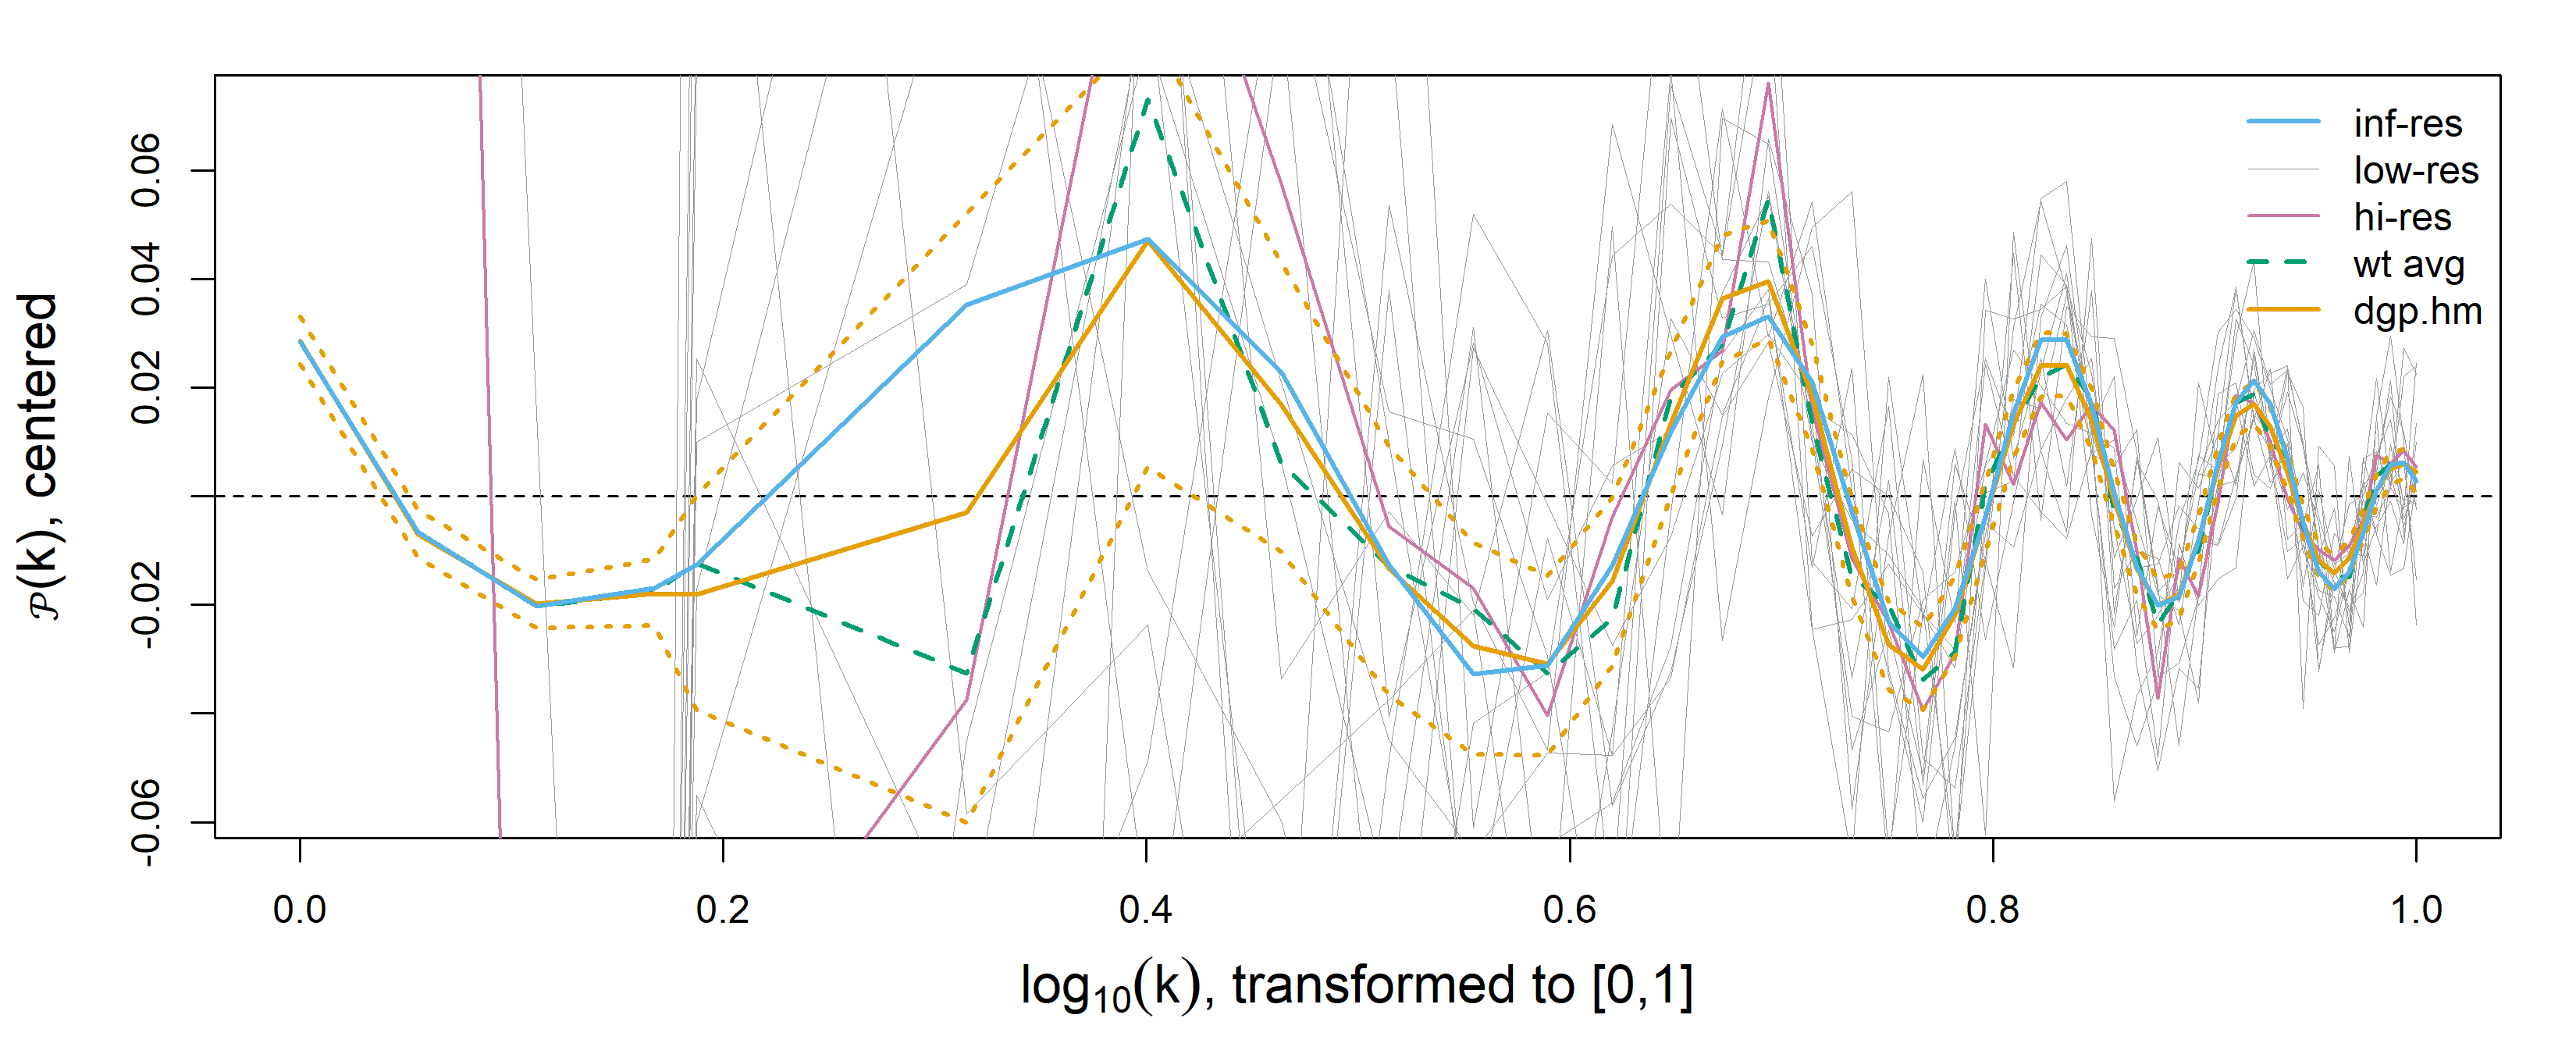
\includegraphics[width=\textwidth]{CAMB_fit_model1.png}
    \caption{Example of DGP.HM model fit for the first batch of model runs from the CAMB data, 
             with LOESS mean term subtracted. We can compare the orange lines 
             (posterior mean and dotted 95\% credible interval) to the light blue line,
             representing the infinite-resolution ``true" spectrum.}   
    \label{fig:fit_camb}
\end{figure}

We use 32 CAMB batches to train the DGP.HM model and reserve the other 32 as a test set.
To imitate the role of the perturbation theory output of Mira-Titan, we anchor estimates of the CAMB
power spectrum at the infinite-resolution for $\log_{10}(k) < -1.7$, and then rely 
strictly on the low- and high-resolution runs for $k$ above this. We take a weighted
average of the CAMB runs and assume heteroskedastic errors in a similar fashion. For the CAMB
data, lengthscale estimates are consistently around $3\times 10^{-7}$, evidence that we
can simplify our covariance structure to contain no spatial dependence 
(compare low-resolution runs of Figure \ref{fig:fit_camb} 
with Figure \ref{fig:plot_data}).

\subsection{Estimating Spectra with Mira-Titan Data}
\label{subsec:mira_fit}

To train our hierarchical model, we initialize our hyperparameter estimates across 
all cosmologies by modeling the first (M001) with 50,000 MCMC runs, and use these 
as initial values for all cosmologies. Specifically, we save the last MCMC 
iteration of $W$, $\theta_w$ and $\theta_S$ as $W_0$, $\theta_{w0}$ and $\theta_{S0}$ 
respectively and use each as starting values for all 111 training cosmology fits, 
where each cosmology is fit with 10,000 MCMC runs (5,000 removed as burn-in and 
every 5th sample is kept, resulting in 1,000 posterior samples).

From these samples, we can estimate and quantify the uncertainty within each 
cosmology's average and latent layer $W$. Figure \ref{fig:plot_fit} shows an 
example of the uncertainty for our posterior mean for the first (of 111) training 
cosmologies; the posterior mean is subtracted in order to visualize this uncertainty. 
Figure \ref{fig:plot_warp} provides elliptical slice samples of $W$ along with the 
average warping. Some departure from stationarity is estimated in the higher $X$ 
(i.e., scaled $k$) values.

\begin{figure}[ht]
    \centering
    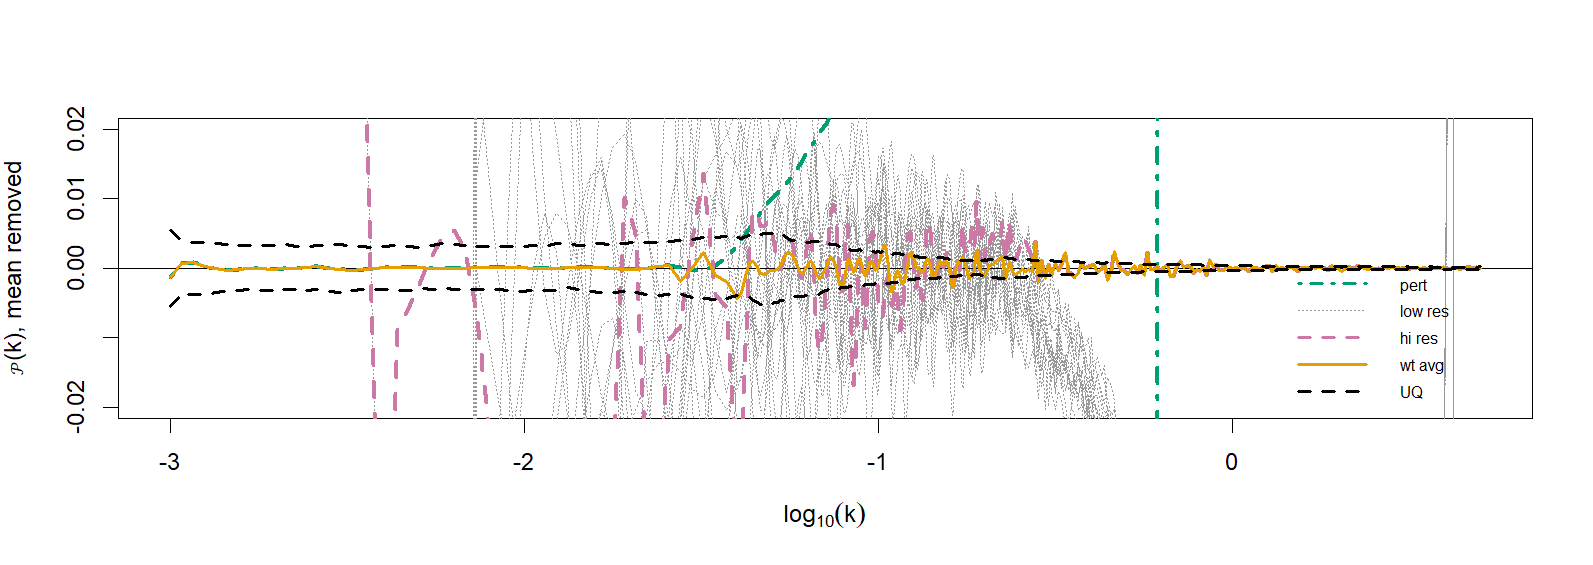
\includegraphics[width=6in]{plot_fit.png}
    \caption{95\% credible intervals for the power spectrum of model 1 (posterior mean 
             subtracted). Plots of the perturbation theory, low-resolution and high-resolution 
             runs are also shown, alongside the weighted average.}
    \label{fig:plot_fit}
\end{figure}

\begin{figure}[ht]
   \centering
   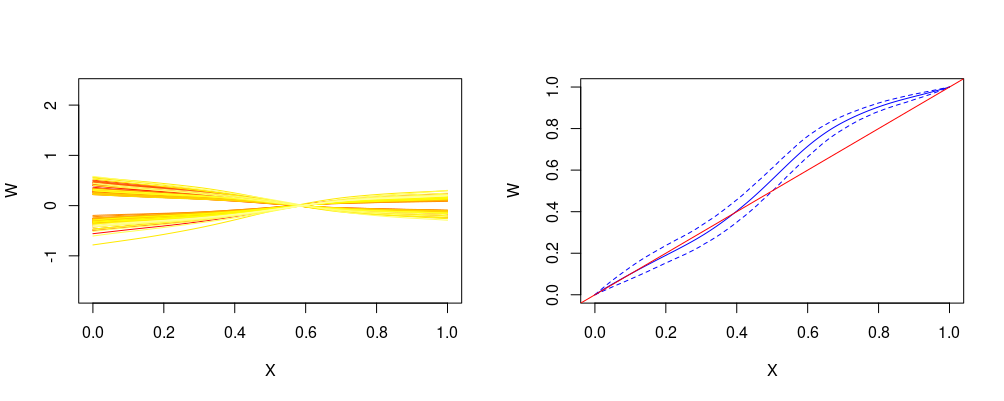
\includegraphics[width=6in]{plot_warp_M001.png}
   \caption{Left: MCMC samples of $W$ for model M001 after burnin and thinning. 
            Right: Corresponding 95\% credible intervals for $W$, where departure 
            from the identity line represents nonstationary behavior.}
   \label{fig:plot_warp}
\end{figure}

\section{Prediction for Unobserved Cosmologies}
\label{sec:pred}

For simplicity, we will denote these eight parameters as $\theta \in \mathbb{R}^8$.


Upon obtaining the posterior means from each of the 111 training cosmologies, this 
section details our second contribution - the use of the Bayesian DGP.HM model 
to predict the curve for held-out cosmologies. This is achieved with modeling the 
weights of different basis functions as GPs.

\subsection{Functional Prediction Model}
\label{subsec:pca}

Here, we begin with a $n \times m$ matrix composed of $m=111$ posterior means, 
each of length $n$, denoted by $\boldsymbol\eta$. To facilitate more efficient estimation, 
we use singular value decomposition \citep[SVD; e.g.,][]{banerjee2014linear}, 
where $\boldsymbol\eta = UDV^T$; $U$ and $V$ are orthogonal matrices of size $n \times n$ 
and $m\times m$, respectively. $D$ is a diagonal matrix containing the singular values. 
For this application, $\boldsymbol\eta$ has rank $r=\text{min}\{m,n\}=111$, which 
determines the number of non-zero elements in $D$. We find an alternative decomposition 
where $\Sigma$ is a diagonal matrix with the non-zero singular values of $\boldsymbol\eta$, 
and $U_1$ and $V_1$ are matrices with orthonormal columns of size $n_\eta \times r$ 
and $m \times r$, respectively. 

Following \cite{higdon2008computer, higdon2010estcosmo}, we equivalently decompose 
$\boldsymbol\eta$ into a principal component (PC) basis matrix 
$B^* = \frac{1}{\sqrt{m}}U_1\Sigma$ along with its corresponding weights 
$W^* = \sqrt{m}V_1$. Without loss of generality, we can perform this decomposition 
after an overall mean trend is removed. If we use $p_\eta < r$ PCs, this will reduce 
$B$ and $W$ to be the first $p_\eta$ columns of $B^*$ and $W^*$ respectively and 
result in an approximation where 

\begin{equation}
    \boldsymbol\eta= UDV^T = U_1\Sigma V_1^T \approx BW^T.
\end{equation}

Figure \ref{fig:mean_PCs_oneW} illustrates this decomposition with the estimated 
mean trend, the principal components contained in $B$, and one example of how the 
weight for the first PC will vary dependent on the first of $p_\theta=8$ cosmological 
parameters contained in $\theta$.

In the following subsections, we consider different modeling strategies for $W$, 
which will influence predictions and sensitivity analyses based on $\boldsymbol\eta$.

\begin{figure}
    \centering
    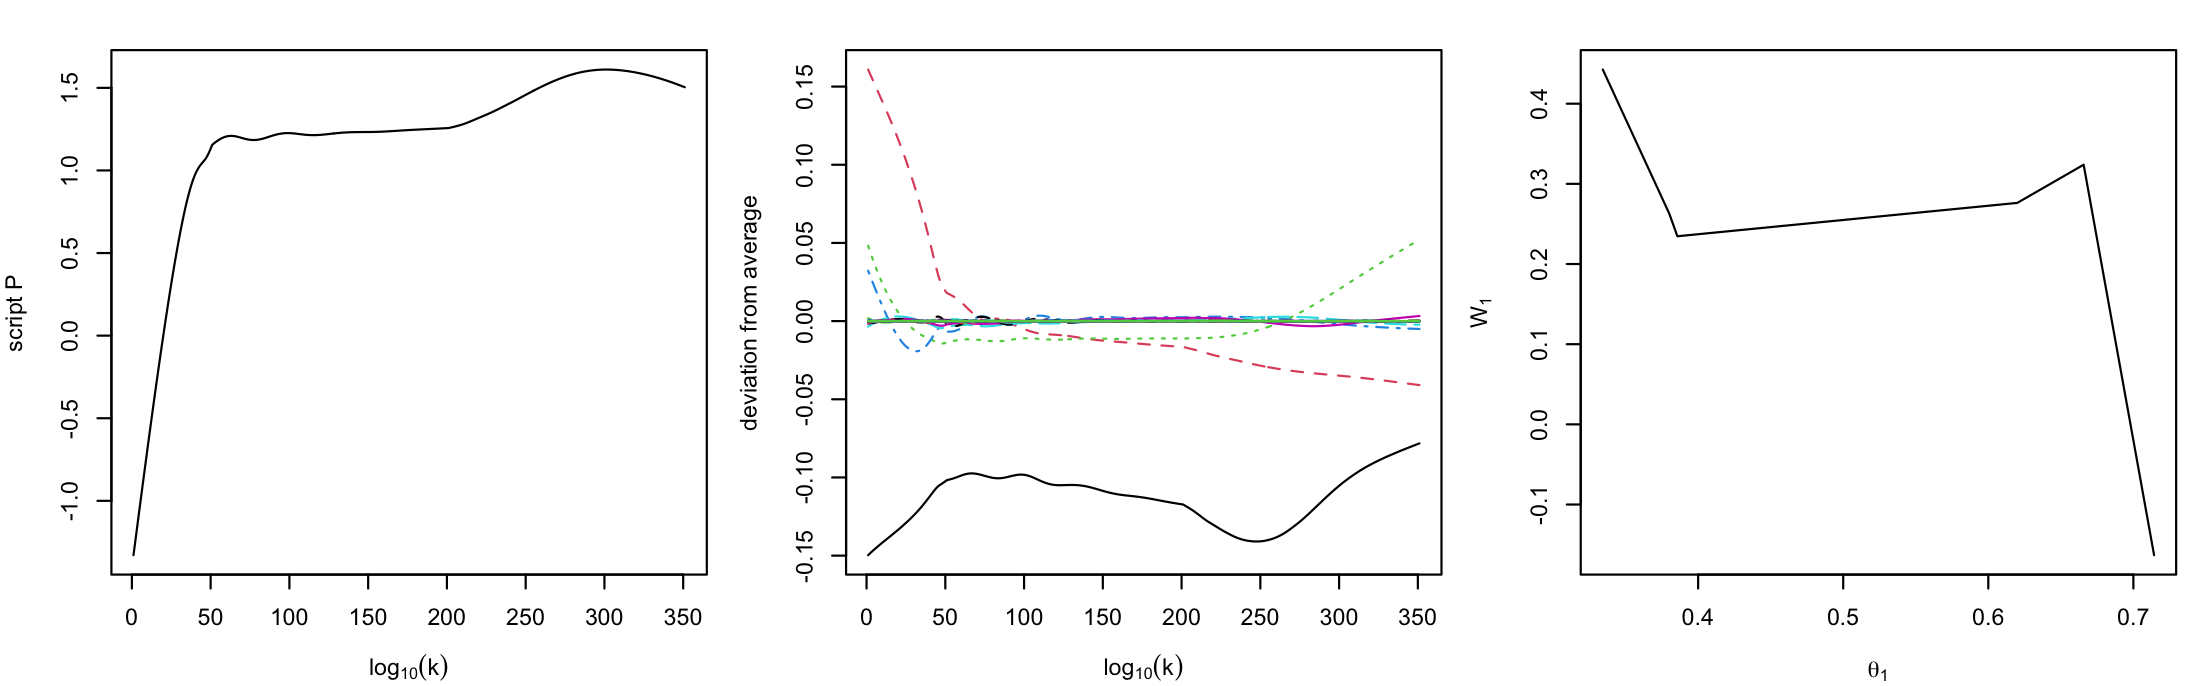
\includegraphics[width=\textwidth]{mean_PCs_oneW.png}
    \caption{The estimated mean trend of the 111 posterior means (left), the principal 
    components contained in $B$ (middle), and an illustration of how the weights 
    for the first PC will change as the first cosmological parameter varies (right) 
    \textcolor{red}{This last plot is wonky because it was made with only the 6 test 
    cosmologies, not a large uniform or FF design, Steve can update this}.}
    \label{fig:mean_PCs_oneW}
\end{figure}



% This is old: switched to SEPIA
% We assume a powered exponential kernel for the Gaussian process and employ 
% \texttt{GPfit} to perform a multi-start gradient based search for GP's hyperparameters 
% \citep{macdonald2015gpfit}. 
In alignment with \cite{heitmann2009coyote} and \cite{higdon2010estcosmo}, we use 
GPs to model the principal components' weights. For direct comparison alongside
\cite{moran2023mira}, we employ a Python implementation of this approach called 
SEPIA \citep{gattiker2020sepia}. \textcolor{red}{Please note: currently show GPfit 
predictions for Mira-Titan Data, NOT SEPIA. The CAMB results are based on SEPIA.}
That is, the $i$th vector of PC weights $w_i(\theta)$, 
$i \in \{1,\ldots,p_\eta\}$, will be modeled as a zero mean GP: 
$w_i(\theta) \sim GP(0, \sigma^2R)$, with

\begin{equation*}
    R_{ij} = \prod_{k=1}^{p_\theta}\exp\left\{-10^{\beta_k}|x_{ik}-x_{jk}|^\alpha\right\}
\end{equation*}

\textcolor{red}{We fix $\alpha=1.95$ and estimate each $\beta_k$ with $k \in \{1,...,p_\theta\}$. 
The above with $R_{ij}$ is based on GPfit; will update this to reflect SEPIA settings later.}
Using these trained GPs from the PCs, we predict the spectra for unobserved cosmologies.

\subsection{Predicting Spectra for CAMB Data}
\label{subsec:camb_pred}

From our 32 posterior means using DGP.HM, these are input into SEPIA in order to predict power spectra
for the 32 test cosmologies. With the infinite-resolution output, we have a sense of the ``best-case" 
predictions we can have (i.e., if we trained with the 32 true power spectra, as opposed to our 
estimated posterior means). In Figure \ref{fig:pca_preds_v_camb}, we see comparisons of the heldout 
infinite resolution alongside two predictions: one based on DGP.HM and the ``best-case" scenario using the
infinite-resolution spectra of the training set. There is a high level of agreement between the pairs
of predictions across cosmologies. Upon comparing MSEs for each of these prediction scenarios 
(Figure \ref{fig:mse_camb}, most are very similar across the two groups (with the two most difficult 
predictions being the exceptions), suggesting that overall DGP.HM is estimating the true spectra 
for each batch well.

\begin{figure}
    \centering
    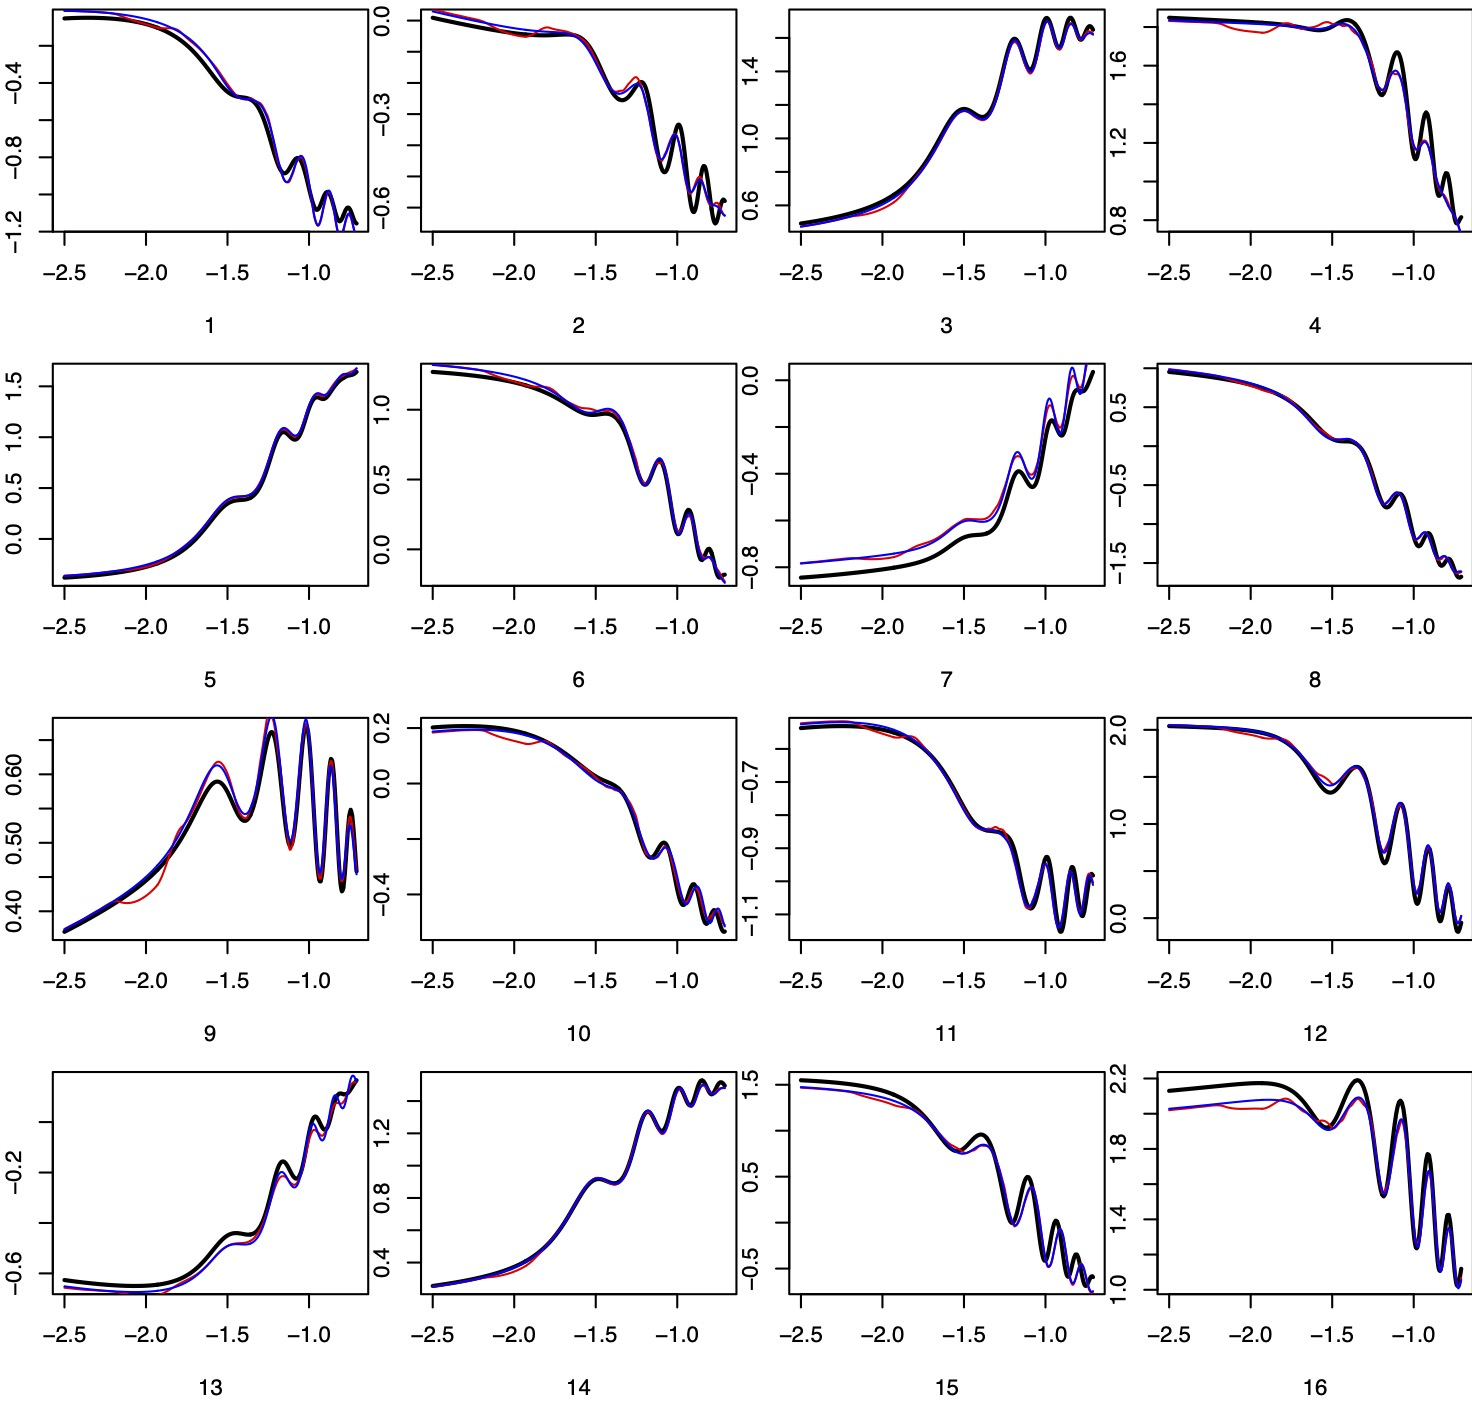
\includegraphics[width=4in]{preds_diff1_4_8.jpg}
    \caption{Predictions for 16 of the 32 test cosmologies after centering and scaling. 
             The interpolated infinite resolution run is shown in black, the prediction 
             (trained on the infinite resolution) is in blue and the prediction from 
             the DGP.HM posterior mean is in red.}   
    \label{fig:pca_preds_v_camb}
\end{figure}

\begin{figure}
    \centering
    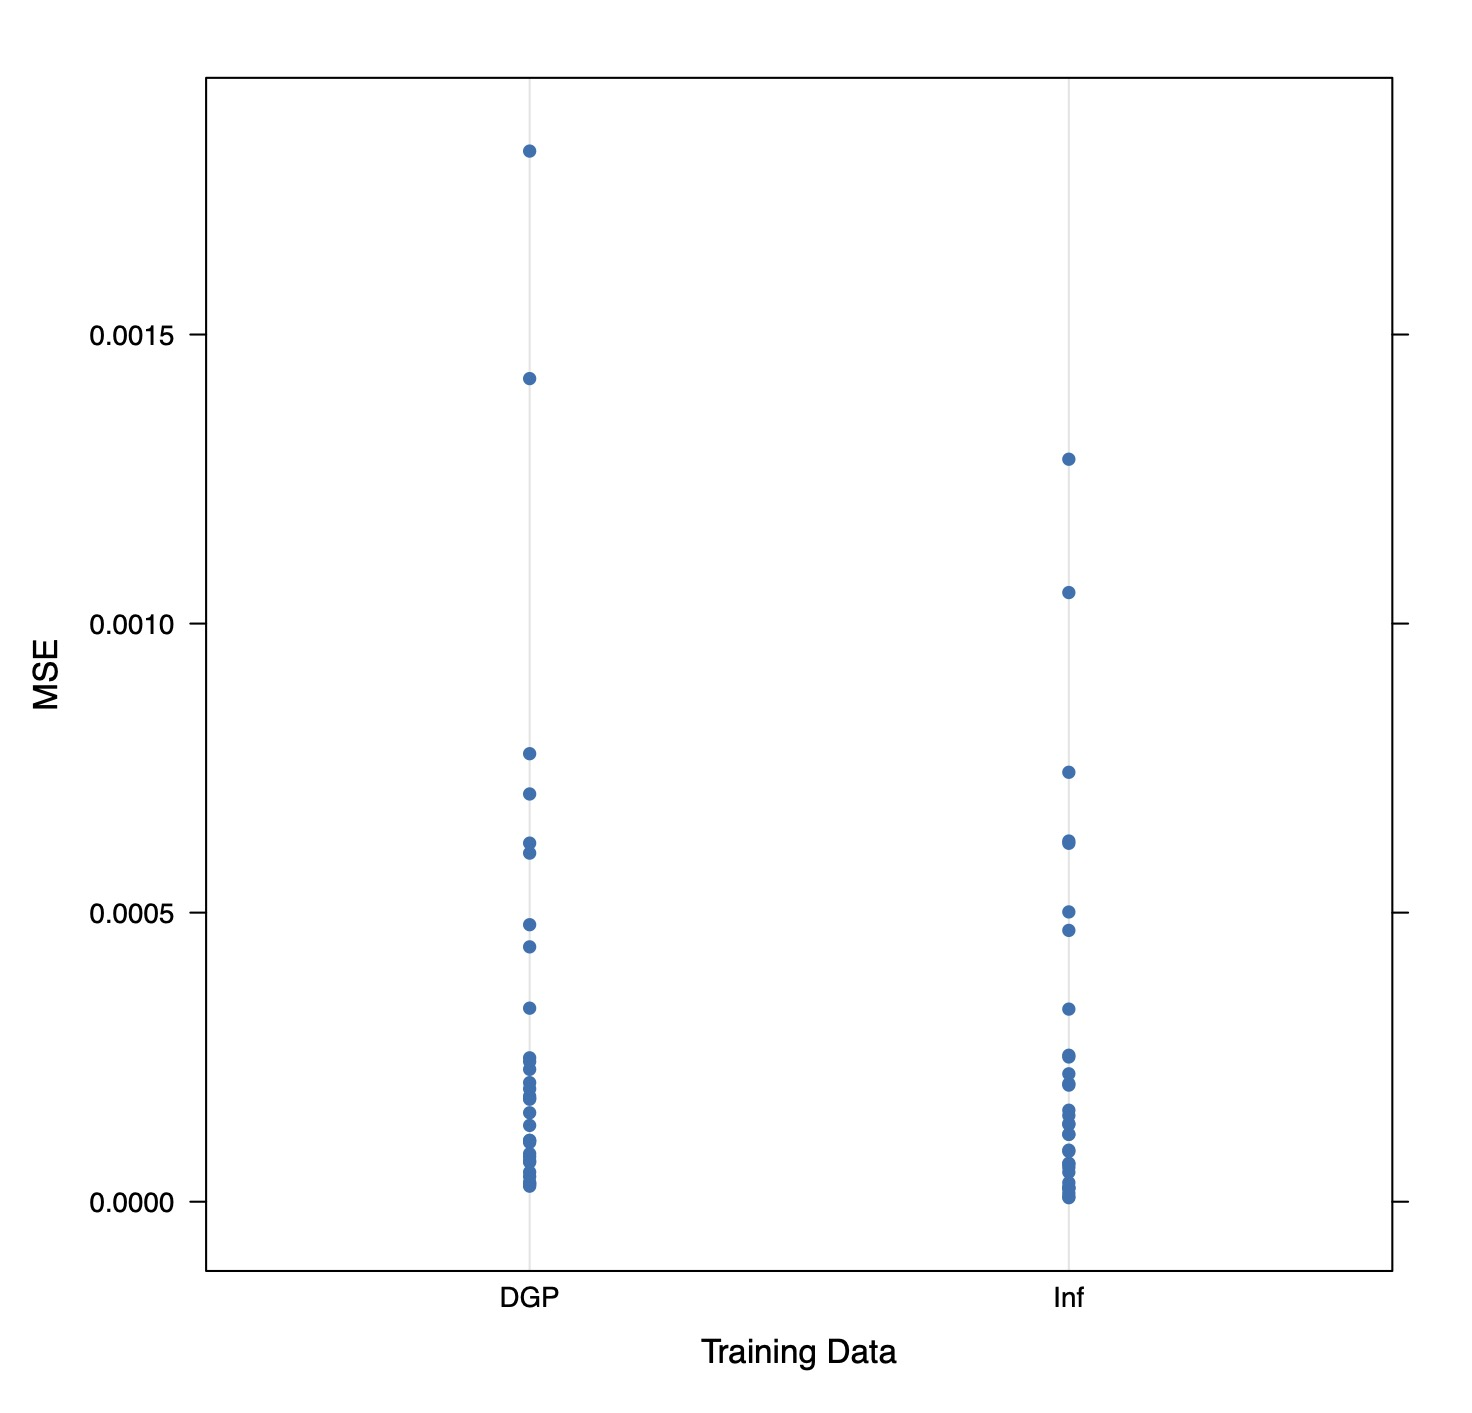
\includegraphics[width=3in]{mse_dot.jpg}
    \caption{Comparison of MSE for CAMB predictions, when training with DGP.HM posterior 
             means (left), and training with the ``true" infinite-resolution spectra (right).}   
    \label{fig:mse_camb}
\end{figure}

\subsection{Predicting Spectra from Mira-Titan Data}
\label{subsec:mira_pred}

Here we show prediction results for 6 held-out cosmologies. We compare our method 
with Cosmic Emu \citep{moran2023mira}, the emulator constructed using the full suite 
of 111 Mira-Titan model runs. Cosmic Emu uses a Bayesian approach where the smooth 
spectrum for each cosmology is modeled with a process convolution on Brownian motion. 
Nonstationarity is permitted through modeling the bandwidth parameter with a process 
convolution as well; this composition is referred to as a deep process convolution 
\citep{moran2024dpc}.

Both Cosmic Emu and DGP.HM are capable of modeling a true underlying functions based 
upon multiple functional realizations, but our approach utilizes DGPs within a 
hierarchical model in lieu of deep process convolutions. After obtaining the estimated 
smooth spectra from the training cosmologies, each method utilizes GPs in order to 
estimate the weights of the PCs from the estimated spectra. Below, we compare prediction 
performance between Cosmic Emu and DGP.HM for the 6 held-out cosmologies. 
\textcolor{magenta}{In addition, we can also predict over a large uniform or full 
factorial design to obtain estimated main effects for each cosmological parameter in 
$\theta$, interactions amongst the $p_\theta=8$ parameters, and decompose the overall 
variation by main effects, two-way interactions, and so on. Should this be included?}

Plots for the average root mean squared error (RMSE) for each prediction method over the 
6 cosmologies and each $k$ value are shown in Figure \ref{fig:plot_rmse_k}. Comparisons 
of the spectrum estimation for training cosmologies are shown as well (using RMSE against 
the weighted average of observations). For predictions, DGP.HM achieves the greatest 
reduction in RMSE in the region where perturbation theory and the low-resolution runs 
are deemed unbiased. For the region where only the high-resolution run is unbiased, 
Cosmic Emu has a lower average RMSE. Over all $k$ values and predictions, DGP.HM has 
an average RMSE of 0.0089 and Cosmic Emu has an average RMSE of 0.0106. Our RMSE is 
lower at 56\% of $k$ values considered. The individual predictions for each method and 
cosmology are shown in Figure \ref{fig:plot_pred_1to6}.

\begin{figure}[ht]
    \centering
    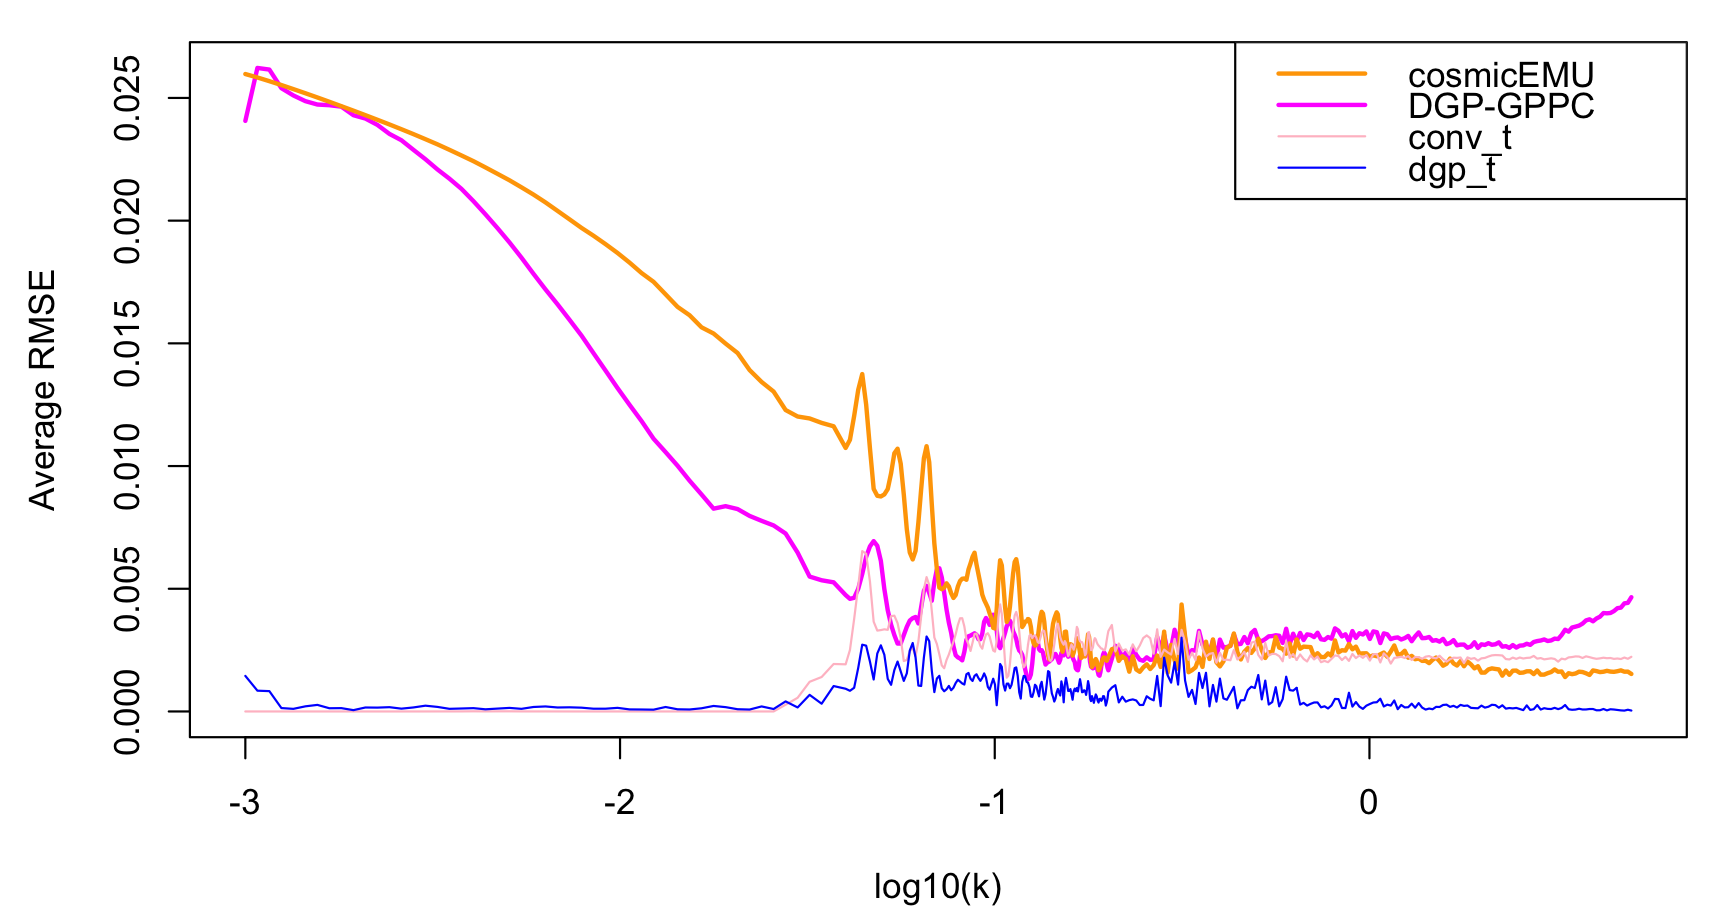
\includegraphics[width=6in]{rmse_by_k.png}
    \caption{Left: Average RMSE of each prediction method across all $k$ values. 
             Right: Average RMSE for each method when using the held-out computer 
             model runs to train the model. In each case, the truth is assumed to 
             be the weighted average of the computer model runs.}
    \label{fig:plot_rmse_k}
\end{figure}

% \begin{figure}[ht]
%     \centering
%     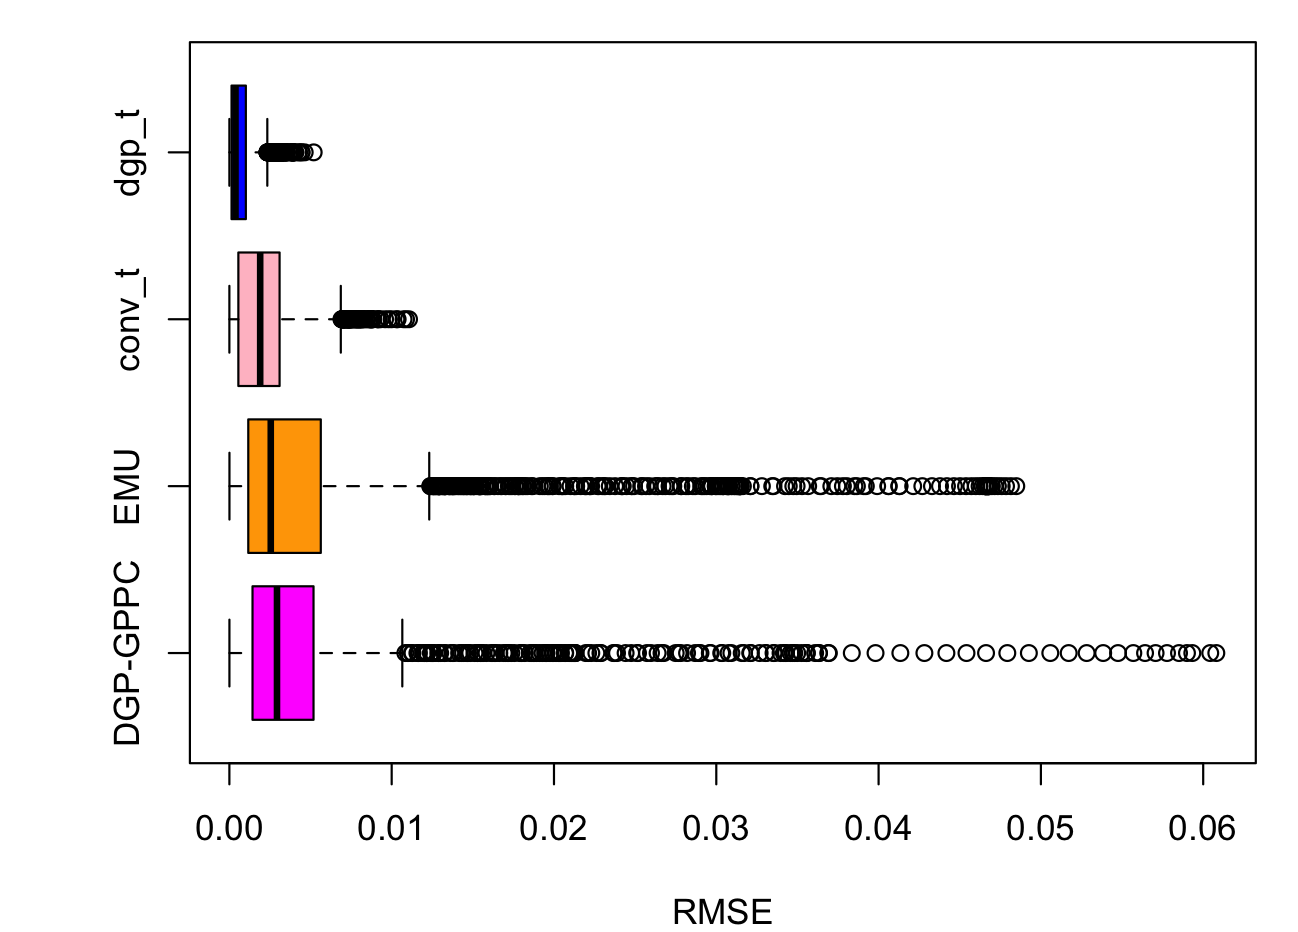
\includegraphics[width=6in]{rmse_box.png}
%     \caption{Boxplot of all RMSEs of each method across all six test models. 
%.             From top to bottom: box plots for our training method, process 
%              convolution training method, Cosmic EMU predictions, and our DGP-PC predictions.}
%     \label{fig:plot_rmse_box}
% \end{figure}

\section{Discussion}
\label{sec:disc}

In this work, we propose a novel Bayesian hierarchical model which utilizes DGPs 
in order to estimate a smooth underlying function from correlated functional observations 
(as cosmological computer model runs). In addition to the compositional form of the DGP, 
we include a third component modeling the correlated errors for each spectrum. 
With all smooth spectra estimated from the training set of 111 batches of model runs, 
we can predict spectra for unobserved cosmologies.

Multiple avenues for future research emerge: in addition to estimating dark matter 
power spectra, batches of hydrodynamical simulations exist, and this method could 
easily be adapted to handle such datasets. Other applications outside of cosmology 
can be explored, wherever multiple functional outputs exist, perhaps with spatial 
correlation (for example, observing multiple tropical cyclone forecasts). More detailed 
sensitivity analyses for the cosmological parameters can be explored to gain insights 
into how each of these parameters interact, and which are most significant. From a 
modeling perspective, changes to the model could include modeling the latent layer 
$W$ jointly across different cosmologies, as well as considering different redshift 
values other than $z=0$. Leveraging a hybrid model between DGP.HM and Cosmic Emu 
may also help to obtain accurate estimates on the lower and higher ends of $k$ values, 
respectively. Additionally, Bayesian smoothing spline ANOVA (BSS-ANOVA) or other methods 
could be compared in addition to DGPs. 

\section{Appendix}
\label{sec:apdx}

\textcolor{magenta}{The different appendices from dissertation as necessary. 
Can also put details of dataset in supplementary material.} 
\textcolor{red}{Fix references as necessary, e.g. Moran et al. 2024.}

\begin{figure}[ht]
    \centering
    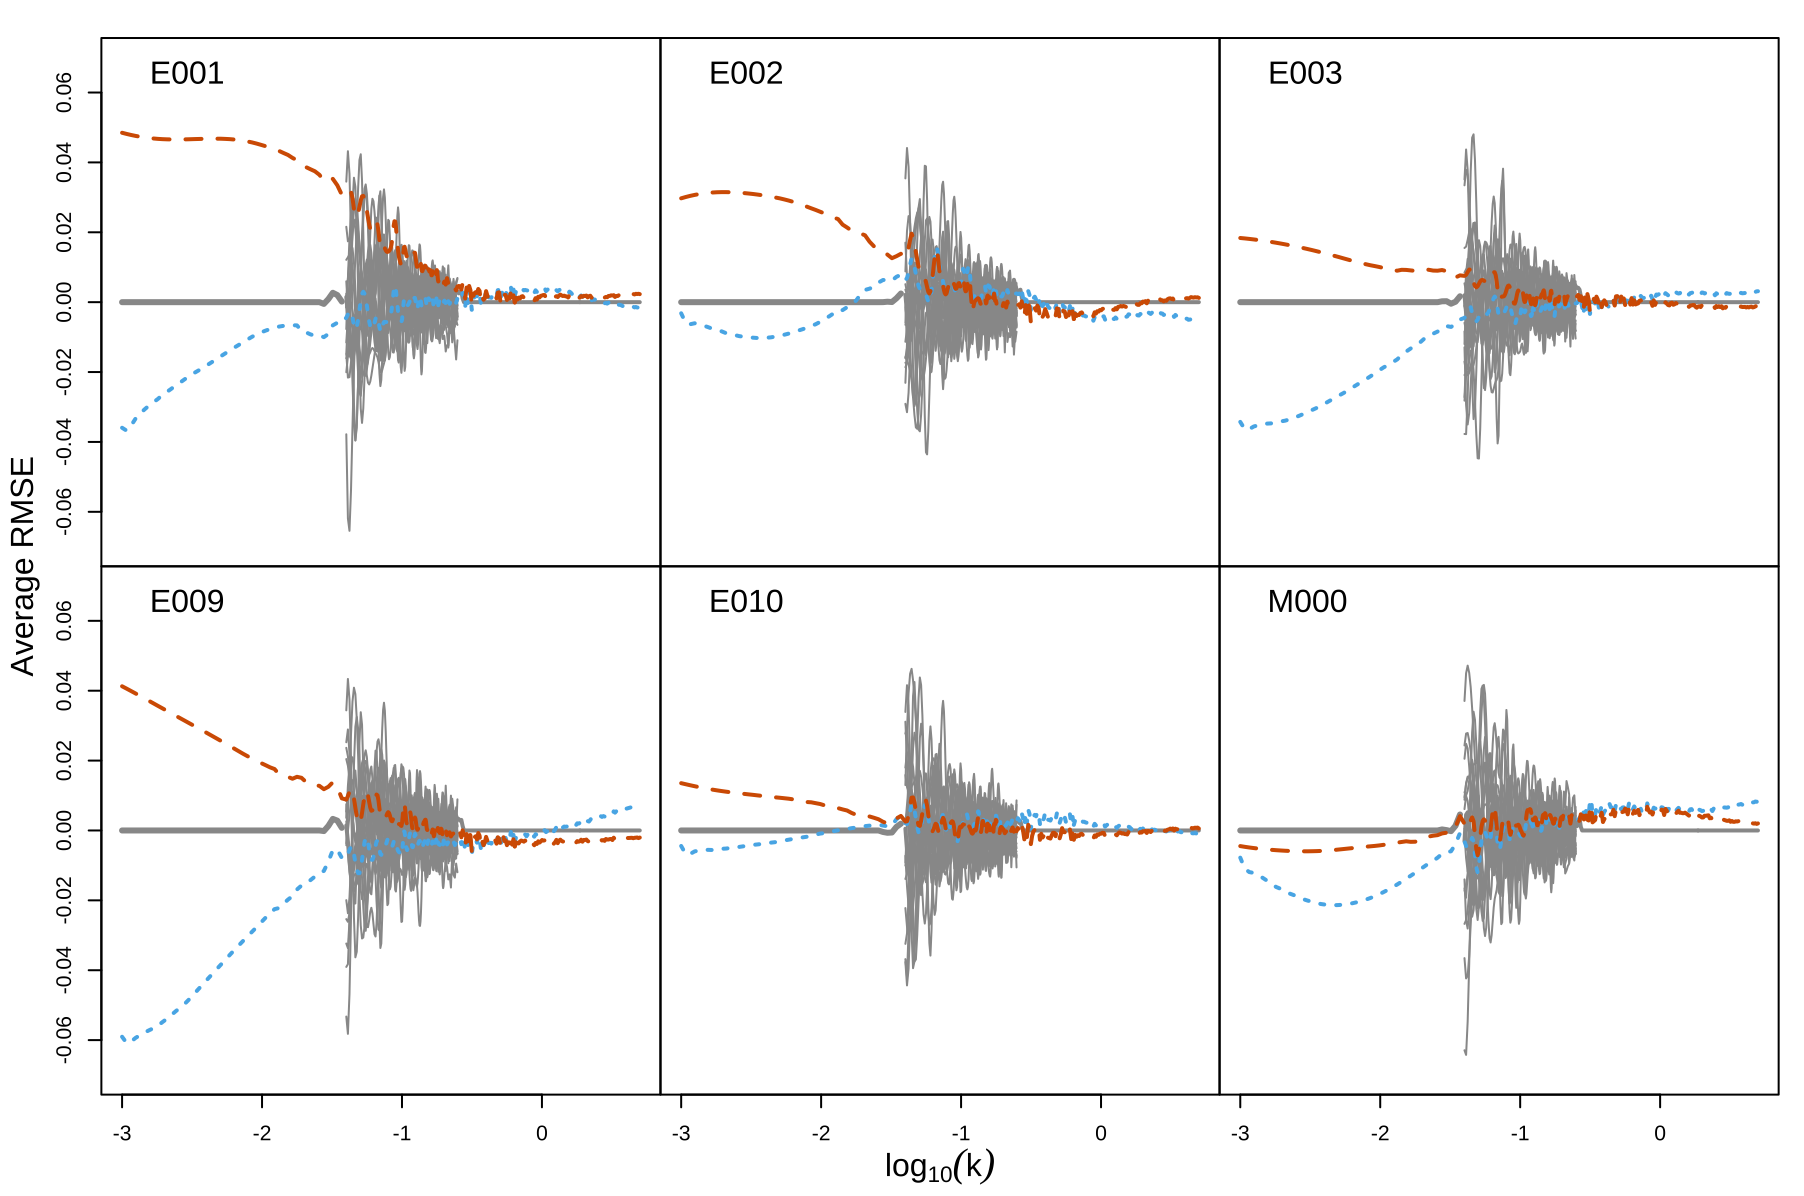
\includegraphics[width=6in]{pred_1to6.png}
    \caption{Results of all six predictions for both methods on the held-out 
    cosmologies (weighted average subtracted). CosmicEMU is dashed, DGP.HM is dotted, 
    and solid gray lines show results of held-out computer model runs.}
    \label{fig:plot_pred_1to6}
\end{figure}

\bibliographystyle{jasa}
\bibliography{references}

\end{document}
